\documentclass{article}

\usepackage[letterpaper, landscape, margin=2in]{geometry}
\usepackage{fancyvrb}
\usepackage[T1]{fontenc}
\usepackage[utf8]{inputenc}

\title{Obligatorisk innlevering 3, høsten 2014, INF3331}
\author{Kristoffer Brabrand <kristrek@student.matnat.uio.no>}
\date{\today}

\begin{document}
\maketitle

\section*{Innledende beskrivelse}
Oppgaven var grei nok å løse når det kom til prinsipper og bruk av python, men matematikken bød på noen utfordringer. Disse var primært knyttet til omregning mellom de ulike fargerommene, avrunding, grenseverdier mv.

De beskrevne oppgavene er løst, men jeg oppdaget for sent at denoise.c opererer på floats og konverterer til en unsigned char (0-255). Ettersom jeg opererer på heltall og runder av underveis har jeg noe større avvik i oppgaven. Dette er beskrevet under den aktuelle oppgaven.

Frontend for de ulike backendene er implementert i denoise.py i roten av oblig3-mappen, og er relativt enkel. Den gjør i korte trekk følgende;

\begin{enumerate}
  \item Parsing av kommandolinjeparametre.
  \item Validerer input.
  \item Henter riktig backend ved bruk av den lokale symboltabellen.
  \item Kaller \verb;denoise_file; på den valgte backenden;
  \begin{enumerate}
  	\item Laster fil inn i liste/numpy.ndarray.
  	\item Utfører denoising og/eller manipulasjon av bildet.
  	\item Skriver bearbeidet fil til målfil.
  \end{enumerate}
\end{enumerate}

Parametrene denoise.py tar vises enklest ved å kalle den med -h som parameter. Outputen som gis når man kaller \verb;denoise.py -h; er vist nedenfor.

%@exec python denoise.py -h

\section*{Oppgave 1: Kodeimport}

Oppgaven er løst ved bruk av et regulært uttrykk som går over flere linjer. Den ser etter et innledende linjeskift før mønsteret for kodeimporten og deretter én eller flere linjer før avslutningstaggen.

Jeg har brukt følgende mønster for å matche kodeimport-instruksjoner;

%@import
\n(%@import ([^\ ]+) (.*))\n
%@

Når mønsteret er funnet i latex-dokumentet blir innholdet i filen det referers til kjørt mot det regulære uttrykket, og det første treffet på dette blir returnert.

Kodeimporten gjøres som en del prosesseringen som gjøres når \verb;prepro.py; kjøres på en latex-fil. Implementasjonen finnes i src/code\_import.py.

\section*{Oppgave 1: Profilering}

Profileringen av de tre implementasjonene er gjort i \verb;test_profiling.py;. Jeg implementerte oppgaven før jeg så kodeeksempelet som ble lagt ut og falt derfor ned på en litt mindre elegant løsning med splitting og offsetting for å finne riktig utvalg fra outputen.

%@import
s = StringIO.StringIO();
ps = pstats.Stats(pr, stream=s).sort_stats('cumulative');
ps.print_stats();

print "\n\n==================================================";
print '{:=^50}'.format(" " + denoiser + " ");
print "==================================================";

print "\n".join(s.getvalue().splitlines()[4:8]);
%@

\subsection*{Resultat fra kjøring}
%@exec python test_profiling.py

Resultatet viser nokså tydelig hastighetsforskjellen mellom den rene python-implementasjonen og numpy-weave/denoise\_c – som er tilnærmet like raske. \verb;cProfile; er et fint verktøy for å profilere og tune python-kode, men er ikke spesielt hjelpsomt hvis målet er å optimalisere C-kode. Da er trolig \verb;gprof; et mer passende verktøy.

\subsection*{Kommentarer til implementasjonen}
Det er imidlertid verdt å nevne at svart-hvit-delen av koden, som er basert på denoise.c har lite rom for optimalisering ettersom den er såpass enkel og bare opererer på array-indekser, mens fargedelen med fordel kunne vært optimalisert.

Spesielt tenker jeg da på at den regner ut HSI-verdier fra RGB for omkringliggende punkter på nytt for hvert punkt. Den burde ha spart på, og gjenbrukt allokerte minneplasseringer for HSI og RGB-verdier og kunne nok med fordel også iterert over og konvertert alle piksler til HSI-verdier før manipuleringen begynte.

\section*{Oppgave 3: Utvidelse til farger}

Utvidelsen til farger er implementert i numpy-weave og hoveddelen av denne logikken finnes i \verb;support_c;-variablen i filen \verb;weave_c.py;.

Metodene \verb;createHSIFromRGB; og \verb;createRGBFromHSI; inneholder utregningen av verdier basert på hhv. RGB og HSI.

Funksjonaliteten er en integrert del av numpy-weave-backenden og brukes dersom formen (shapen) på dataene som er importert med numpy er med tre dimmensjoner, à la (375, 500, 3). Siden arrayet blir gjort om til et endimmensjonalt array i weave brukes antallet componenter/kanaler til å beregne indexen for hver pixel i C-implementasjonen, slik som her;

%@import
// Calculate index of current pixel
current = (i * width + j) * channels;
%@

(Variablene i og j svarer til hhv. raden og kolonnen i bildet.)

\section*{Oppgave 4: Lineær manipulering}

Oppgaven som gikk på lineær manipulering var ikke så godt beskrevet i oppgaven, men jeg har tatt utgangspunkt i at det er et positivt eller negativt tall som adderes til den aktuelle komponenten/kanelen på alle punkter i bildet.

Parametrene for å manipulere verdiene i bildet sendes med til frontend som vist i hjelp for denoise.c;

%@input
--lr N  Amount to add to or remove from the R channel (RGB).
--lg N  Amount to add to or remove from the G channel (RGB).
--lb N  Amount to add to or remove from the B channel (RGB).
--lh N  Amount to add to or remove from the H component (HSI).
--ls N  Amount to add to or remove from the S component (HSI).
--li N  Amount to add to or remove from the I component (HSI).
%@

Manipulering av flere kanaler kan gjøres samtidig og all manipulering skjer etter evt. denoising. Ettersom konvertering til/fra HSI er krevende sjekkes det om det skal gjøres manipulering av noen av HSI-komponentene, og evt. konvertering gjøres da. RGB krever ikke noen konvertering ettersom verdiene i arrayet er RGB-verdier.

Det er implementert sjekker for å sørge for at ingen manipulering fører til verdier som er utenfor grensene som gjelder for de ulike komponentene.

\subsection*{Eksempel på lineær manipulering}
\begin{figure}[!h]
\centering
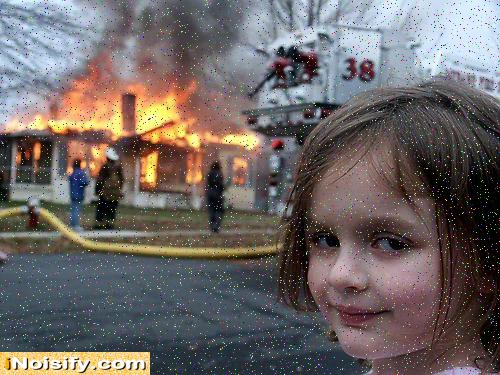
\includegraphics[width=90mm]{disasterbeforecolor}
\caption{Original image}
\end{figure}

\pagebreak

\begin{figure}[!h]
\centering
%@exec
python denoise.py assets/disasterbeforecolor.jpg \
report/images/nw-color-02-5-100-02.jpg --kappa=0.2 --iter=5 --lr=100 --ls=-0.2
%@
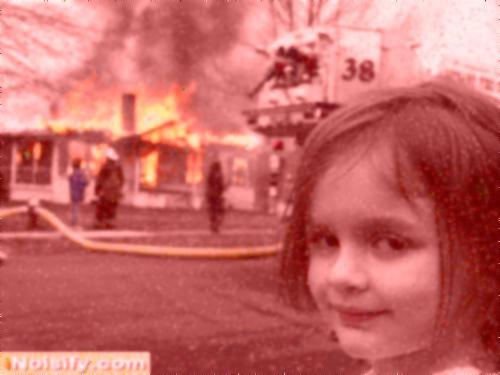
\includegraphics[width=90mm]{nw-color-02-5-100-02}
\caption{Denoised with numpy-weave, kappa=0.2, iter=5, r=100, s=-0.2}
\end{figure}

\pagebreak

\section*{Oppgave 5: Frontend}

Output fra frontend er vist allerede, så jeg gjentar ikke det, men et par andre ting er verdt å nevne.

\subsection*{Timeit i frontend}
Det står nevnt i opgaveteksten at det skal være mulig å skru \verb;timeit;-modulen av/på i frontend. Med en tanke om fordeling av ansvar (separation of concerns) i bakhodet mener jeg at det tilfører lite verdi å ha timeit-funksjonalitet i frontenden ettersom man skjeldent bruker mer enn én backend samtidig likevel.

Jeg valgte derfor, som tidligere beskrevet, å implementere hastighetssammenlikning i en separat fil; \verb;test_speed_test.py; og output fra denne er vist tidligere.

\subsection*{eps-parameter til frontend}
Jeg forsto rett og slett ikke hvorfor denne skulle være et parameter til frontend og valgte til slutt å ta den bort. Den er tatt med som første og eneste parameter til sammenlikningstesten som genererer og sammenlikner verdier i bilder (\verb;test_file_comparison.py;).

\section*{Oppgave 7: Kompilering av preprosessert fil}

Kompilatoren er så begrenset i omfang at jeg valgte å implementere den som én enkelt fil. Kompilatoren starter en subprosess av \verb;pdflatex; ved hjelp av \verb;subprocess.Popen;

Som standard kjøres \verb;pdflatex; i nonstopmode ved at interaction-flagget settes til nonstopmode. Dette kan deaktiveres ved å sette interactive-flagget når compile.py-scriptet kalles.
Output fra compile.py går – som i \verb;pdflatex; – som standard til den samme mappen som latex-filen som prosesseres ligger i. Dette kan overstyres ved å kalle compile.py med et destination-parameter.

Alle parametre til compile.py vises enkelt ved å kalle \verb;python compile.py -h;. Dette gir følende output;

%@exec python compile.py -h

\end{document}
